

\practic


\section{Архитектура}
Цель – разработать высокопроизводительный систему кластеризации документов, которая принимаем документ (PDF, DOCX), генерирует кластеры для извлеченных текстовых данных и сохраняет результат в графовом виде. 

Как было упомянуто в теоритической части, приложение реализовано с использованием микросервисной архиктеруры. Подробно расскажем о ней:

\begin{figure}[h!]
    \centering
    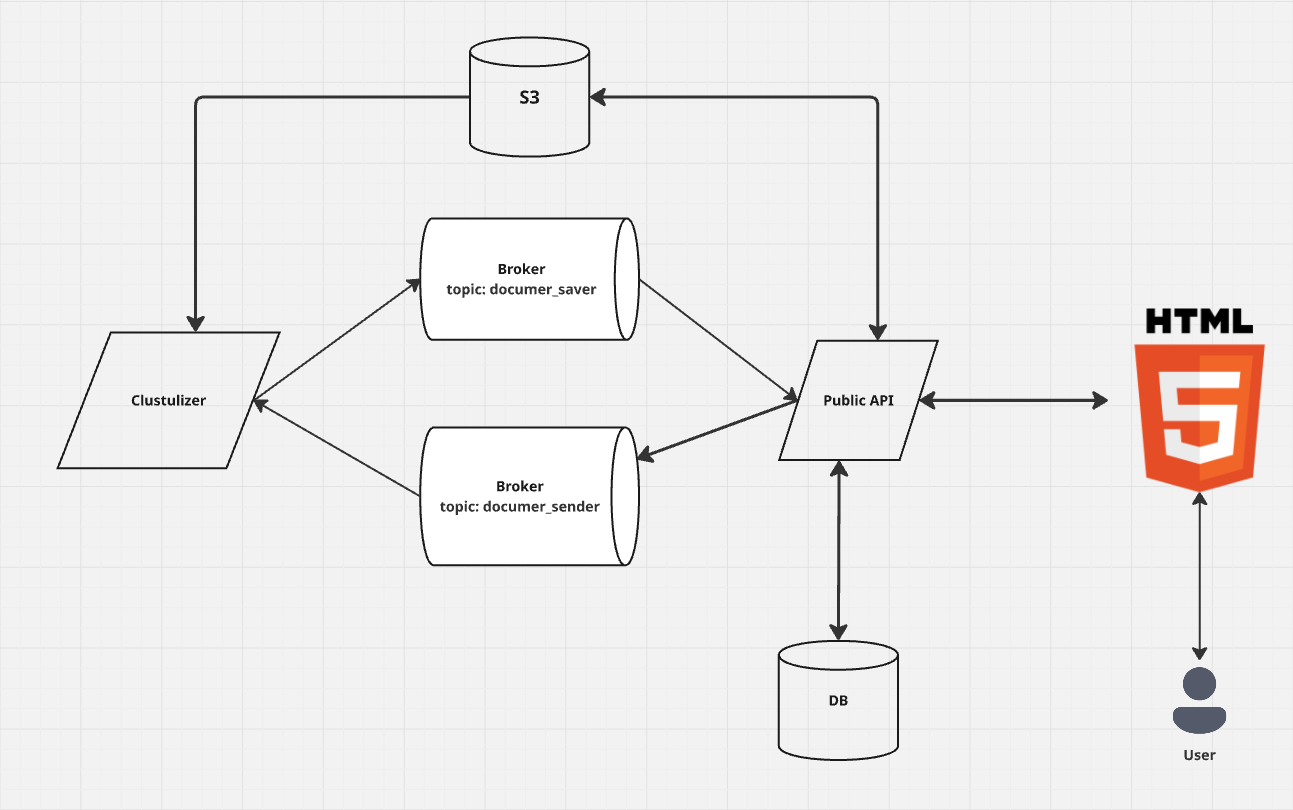
\includegraphics[width=1\textwidth]{styles/diploma/inc/microservice2.png} 
    \caption{Архитектура приложения}
    \label{fig:example}
\end{figure}
Система состоит из 5 компонентов:
\begin{itemize}
    \item S3 (Simple Storage Service);
    \item Broker;
    \item DB;
    \item  Сервис  Public AP;
    \item Сервис  Clusterizer;
    \item Пользовательский интерфейс.
    
  \end{itemize}
\subsection{Логика приложения}
\begin{enumerate}[label=\arabic*)] 
\item Пользователь загружает файл в графическом интерфейсе;
\item Пользовательский интерфейс совершает AJAX-запрос и ждет ответа сервера;

\item Сервер возвращает уникальный ID, который frontend сохраняет в виде cookie данных. Запускается периодическяа фукнция, делающая с заданным интервалом AJAX-запрос к Public API для получния статуса обработки документов;

\item Файл попадает в Public API. Добавляется запись в  DB о создании новой заявки на обработку. Файл отправляется в broker на топик processing, а также сохраняется в хранилище S3;
\item Clustulizer получает сообщения из топика processing , обрабатывает  и передает результат в топик save;
\item Public API читает топик брокера save, получает результат обработки  и сохраняет его в БД;
\item Пользователь получает результат в графическом интерфейсе.
\end{enumerate}

\section{Компоненты приложения}
Подбробнее расскажим об каджой компоненте

\subsection{S3}

В проекте хранилище S3 необоходимо для управления файлами пользователя. Система не ограничивает размер входных данных, поэтому было решино использовать данную технологию.

Как было отмечено в теоретической части, S3 — это всего лишь API, а значит, любой провайдер может реализовать совместимый способ хранения данных. В рамках архитектуры моего проекта я рассматриваю несколько поставщиков облачных хранилищ, каждый из которых предлагает S3-интерфейс с различными характеристиками.

\begin{itemize}
    \item \textbf{Yandex Cloud:}'
    
    Российская облачная платформа с развитой экосистемой сервисов, включая облачное хранилище с полной поддержкой S3 API. Отличается стабильной производительностью, хорошей документацией и активной технической поддержкой. Локализована, соответствует российским требованиям по хранению данных и регулярно обновляется. Yandex Object Storage легко интегрируется с микросервисной архитектурой и поддерживает IAM, версионирование, классы хранения и шифрование на стороне сервера.
    \item \textbf{СберCloud:}
    
    Платформа от Сбера, ориентированная на корпоративный сектор и государственные организации. Также предоставляет S3-совместимое хранилище, но часто предполагает более сложную бюрократическую процедуру подключения и настройки. Имеет сильную интеграцию с инфраструктурой Сбера, но менее гибка и медленнее обновляется по сравнению с конкурентами.
    \item \textbf{VK Cloud:}
    
    Ещё один крупный российский провайдер с поддержкой S3. VK Cloud предлагает интересные тарифы и технически надёжную реализацию. Однако экосистема менее развита, чем у Яндекса, а документация и поддержка не всегда оперативны.
   
  \end{itemize}

  Хотя каждый из представленных провайдеров предлагает базовую поддержку S3-интерфейса, Yandex Cloud наиболее полно сочетает в себе техническую зрелость, простоту интеграции, гибкие тарифы и совместимость с современными DevOps-инструментами. В контексте микросервисной архитектуры с ML-компонентами, где важны скорость, стабильность и автоматизация, выбор очевиден — Yandex Object Storage.

\subsection{Broker}

Broker является очередью сообщений. В роли очереди используется RabbitMQ.
Данная компонента система необходимо для передача данных от одного сервиса к другому. 

Приложение должно удолетворять критериям скорости и наджености. В системе Broker решает сразу оба:
\begin{itemize}
    \item \textbf{Надежность}. Если некоторый запрос зависнит,потеряет и т.п, то он сохранится в памяти брокера, поэтому  клиенты получать результат практически в 100\% случаев
     \item \textbf{Скорость}. Брокер способен балансировать пришедшие на него сообщения, то есть он будет выбирать только доступные репликации другого микросервиса, что особенно важно для пользовательского опыта.
\end{itemize}
\subsection{DB}

DB представляет собой объектно-реляционную базу данных. Благодаря выбранной архитектуре   микросервисов( о которой погорим далее), можно выбрать любую базу данных.

Я остановился на PostgresQL. Кратко пройдусь по причинам ее выбора:
\begin{itemize}
\item  \textbf{Поддержка сложных запросы, транзакции и индексацию}. Любая система, подразумевающая себя высоконагруженной, обязательно должно иметь следущих список технологий.Особеноно важным является индекс.

Индексы в PostgreSQL — это важный механизм оптимизации, который позволяет ускорить выполнение запросов за счёт сокращения количества просматриваемых строк в таблице. Вместо полного прохода по таблице (что может занимать значительное время при большом объёме данных), индекс позволяет базе быстро определить, где находятся нужные записи. PostgreSQL поддерживает разнообразные типы индексов (B-tree, Hash, GIN, GiST и другие)
\item \textbf{Поддержка JSON}. Позволяет удобно хранить и обрабатывать как структурированные, так и полуструктурированные данные в одной базе. 
\end{itemize}

База данных содержит 2 таблицы  - request и file.
\begin{table}[H]
\centering
\caption{Структура таблицы \texttt{request}}
\begin{tabular}{|l|l|l|}
\hline
\textbf{Поле} & \textbf{Тип данных} & \textbf{Описание} \\
\hline
\texttt{id}          & UUID            & Первичный ключ \\
\texttt{result}      & JSONB           & Результат запроса (в JSON) \\
\texttt{status}      & varchar(50)     & Статус запроса \\
\texttt{created\_at} & TIMESTAMP       & Дата создания (по умолчанию \texttt{now()}) \\
\texttt{updated\_at} & TIMESTAMP       & Дата обновления (по умолчанию \texttt{now()}) \\
\hline
\end{tabular}
\end{table}

Таблица request необходима для учета пользователей запросов  обработки документов. Подробно расскажу о каждом поле:
\begin{itemize}
\item  \textbf{id}. Уникальный индификатор. Необходим для корректной работы пользовательского интверфейса;
\item  \textbf{result}. Содержит результат обработки документов кластеризатором;
\item \textbf{status}. Показывает состояние запроса в данный момент;
\item \textbf{created\_at}, \textbf{updated\_at}. Метаданные, необходимые для аналитики и отслеживания работы системы. 

Поле \textbf{created\_at} фиксирует момент создания записи, а \textbf{updated\_at} — время последнего изменения. Эти данные позволяют анализировать активность, выявлять задержки и отслеживать возможные проблемы в системе.
\end{table}


\begin{table}[H]
\centering
\caption{Структура таблицы \texttt{file}}
\begin{tabular}{|l|l|l|}
\hline
\textbf{Поле} & \textbf{Тип данных} & \textbf{Описание} \\
\hline
\texttt{id}   & UUID          & Первичный ключ \\
\texttt{type} & varchar(30)   & Тип файла \\
\texttt{key}  & varchar(100)  & Ключ \\
\texttt{title}& varchar(255)  & Название \\
\hline
\end{tabular}
\end{table}

Таблица file необходима для учета файлов для даленьшего удобного скачивания нужного файла. Подробно расскажу о каждом поле:
\begin{itemize}
\item  \textbf{id}. Уникальный индификатор. Необходим для корректной работы пользовательского интверфейса;
\item  \textbf{type}. Содержит формат файла(docx или pdf);
\item \textbf{status}. Показывает состояние запроса в данный момент;
\item \textbf{key}. Индификатор файла, по которому он сохранен в S3
\item \textbf{title}. Полученное название файла

Поле \textbf{created\_at} фиксирует момент создания записи, а \textbf{updated\_at} — время последнего изменения. Эти данные позволяют анализировать активность, выявлять задержки и отслеживать возможные проблемы в системе.
\end{itemize}

\subsection{Сервис Public AP}
Public API является легковесным HTTP-сервером. Данный компонент является своего рода входного узла.  Он не влючает в себя тяжелую CPU Bound нагрузку, а лишь I/O Bound. 
Все поользовательские запросы обращаются именно к нему, а Public API общается с другими сервисами.

Public API использует следующие технологии:
\begin{itemize}
\item  \textbf{Golang}. Компилируемый язык, обеспечивающий высокую скорость чтения/записи. Облагает встроенными структурами данных (такими как горутины и каналы), которые позволяют эффективно управлять параллелизмом и конкуренцией, что особенно важно для микросервисных архитектур

Для конкретнно данного микросервиса можно было выбрать любой другой язык, но философия Golang изначально подразумевает микросервисную архитектуру, поэтому эта технология более подхоядщяая, нежели другие.
\item  \textbf{Fiber}. Cовременный высокопроизводительный легковесный веб-фреймворк для Golang. Разработан для создания микросервисов;
\item \textbf{pgxv5}. драйвер-библиотека с  взаимодействия с PostgreSQL для языка Golang.

\end{itemize}

Public API написан с использованием луковой архитектуры - паттерна, который направлен на улучшение гибкости, тестируемости и устойчивости приложения к изменениям. Он помогает отделить бизнес-логику от инфраструктурных деталей, минимизируя связность между компонентами системы.

\begin{figure}[H]
    \centering
    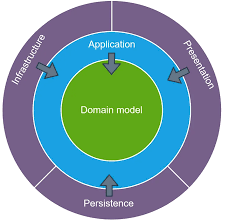
\includegraphics[width=0.5\textwidth]{styles/diploma/inc/onion1.png} 
    \caption{Устройство луковой  архитектуры}
    \label{fig:example}
\end{figure}

Микросервис состоит из 3-х слоев:
\begin{itemize}
\item  \textbf{Storage}
\item  \textbf{Service}
\item  \textbf{Handler}
\end{itemize}
Подробно расскажем о каждом из них

\subsubsection{Storage}
Отвечает за взаимодействие с базой данных.
Все методы имеют примерно одинаковую структуру:
\begin{itemize}
\item Аргумент params содержит данные, необходимые для совершения запроса к БД. Это могут быть как данные для изменения, так фильтры для возвращения данных.
\item  Запрос к базе данных через ранее инициализированный клиент PostgreSQL (метод client.Query).
Клиент представляет собой преднаписанную структуру, позволяющую совершать транзакционные запросы, что череезвычно важно в подобных проектах.
\item  Получение и преобразование данных (pgx.CollectOneRow или pgx.CollectRow и requestToEntity соответсвенно )
\end{itemize}



\begin{figure}[H]
    \centering
    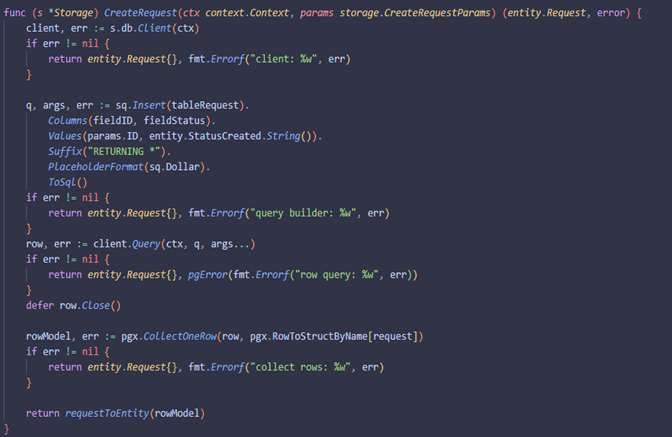
\includegraphics[width=1\textwidth]{styles/diploma/inc/storage1.png} 
    \caption{Пример метода слоя Storage -  функция создания пользовательского запроса.}
    \label{fig:example}
\end{figure}

\subsubsection{Service}

Содержит основную бизнес-логику приложения.

Бизнес логикой может являться как полноценный алгоритм(например,как на рисунке 12. В дополнению к предыдуему пункту видно использование тракзакций), так и обертка вокруг другого слоя для поддержания слоистой архитектуры.

Service использует методы слоя Storage. Важно отметить, что Service получает интерфейс Storage, то есть он не знает какая реализация лежит за этим интерфейсом. Это позволяет пластично менять технологии проекта, не затрагивая основную бизнес логику.



\begin{figure}[H]
    \centering
    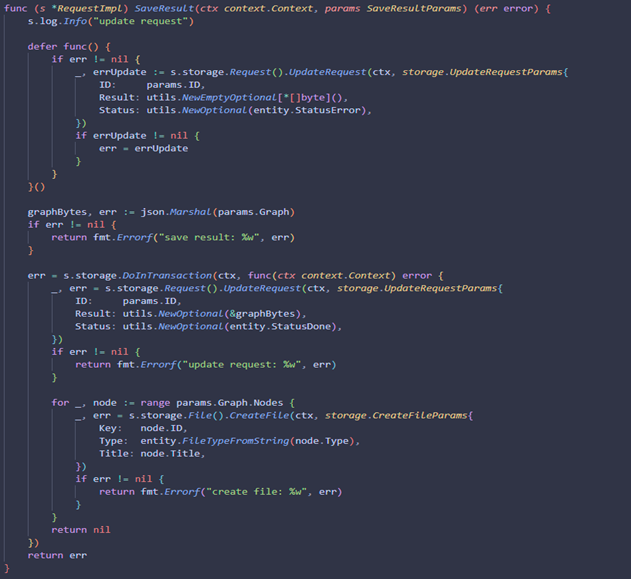
\includegraphics[width=1\textwidth]{styles/diploma/inc/service1.png} 
    \caption{Метод SaveResult}
    \label{fig:example}
\end{figure}

\begin{figure}[H]
    \centering
    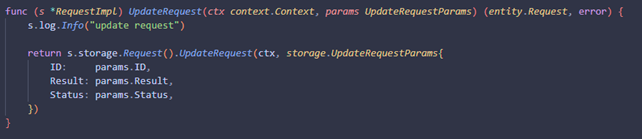
\includegraphics[width=1\textwidth]{styles/diploma/inc/service2.png} 
    \caption{Метод UpdateRequest}
    \label{fig:example}
\end{figure}

\subsubsection{Handler}
Handler - dходная точка для обработки пользовательских запросов. Чащего всего она предславляет собой методы, вызывающиеся при сетевом запросе.
В моем случае - это HTTP запросы.

В слое Handler происходит “склейка” ранее написанных  методов в слое Service. На рисунке 14 представлен метод загрузки пользовательских файлов. Стоит рассказать о каждой шаге в этом методе:

\begin{enumerate}[label=\arabic*.]
\item Строки 46-48, структура \textbf{uploadFilesRequest}  – требуемый вид запроса для метода;
\item Строки 50-52, структура \textbf{uploadFilesResponse}  – требуемый вид ответа для метода;
\item Строки 57-62, метод \textbf{h.getUploadFilesFromForm}  – обработка входных данных в понятном для языка виде;
\item Строки 64-72, метод \textbf{h.requestSrvc.CreateRequest }  – создание в БД записи нового пользовательского запроса;
\item  Строки 73-85, метод \textbf{h.s3Srvc.Upload}  - Создание уникальных индификаторов для файлов и их сохранение в хранилище S3  с помощью метода h.s3Srvc.Upload; 
\item  Строки 86-94, метод \textbf{h.documentSrvc.SendDocumentNames}  - отравка уникальных ключей файлов для дальнешней обработки на брокер сообщений.
\end{enumerate}

\begin{figure}[H]
    \centering
    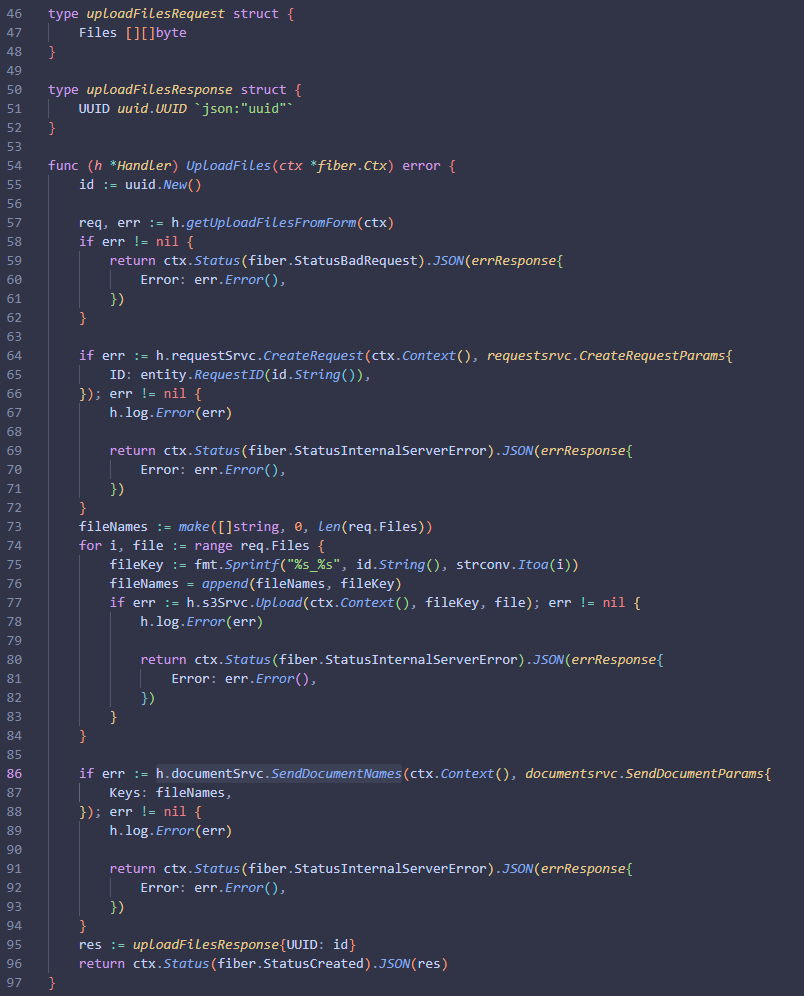
\includegraphics[width=1\textwidth]{styles/diploma/inc/handler1.png} 
    \caption{Метод UploadFiles для загрузки пользовательских файлов}
    \label{fig:example}
\end{figure}

\subsection{Сервис Clustulizer}
Clustulizer -  модуль кластеризации документов, который принимаем документ (PDF, DOCX), генерирует кластеры для извлеченных текстовых данных и возвразает результат в графовом виде

Clustulizer использует следующие технологии:
\begin{itemize}
\item  \textbf{Python} - нтерпретируемый язык,широко используется в задачах анализа данных и машинного обучения. Мой выбор пал на него в виду того, что большиство библиотек для анализа данных и кластеризации написаны именно на нем.


\item  \textbf{Sentense Tranformers }.– высокоуровневая библиотека для python, на основе transformers, предназначена для генерации эмбеддингов слов, предложений и целых документов для последующего семантического поиска похожих, может работать с большим количеством моделей, в данной работе выбрана SBERT-LARGE-NLU-RU.
\item \textbf{Модель SBERT-LARGE-NLU-RU}– модель, которая наиболее эффективна среди других моделей, обученных на русских текстах.
\item \textbf{FastAPI }– современный высокопроизводительный асинхронный веб-фреймворк для python. Его выбор обусловлен его быстротой, асинхронностью, строгой типизаци (он использует pydantic), быстротой написания кода, а также автоматической генерации документации swagger, вместе с ним используется uvicorn – легковесный, высокопроизводительный ASGI-сервер.
\end{itemize}

Clustulizer использует такую же слоистую архитектуру, как Public API.
Рассмотрим каждый слой.
\subsubsection{Storage}
Clusterlizer не взаимодействует с БД, поэтому этот слой пустой. Связано это с тем, что микросервисная архитектура требуют, чтобы у каждого сервиса была своя база данных, иначе может возникнуть сильная связанность, и смысл самой архитектуры потеряется. Все записи в базу данных выполняет сервис Public API.
\subsubsection{Service}

 Слой Service состоит из 3 классов: Converter, S3, ClusterGraphBuilder, но отдельное внимание обратим лишь на ClusterGraphBuilder, так как первые 2 по сути являются обертками вокруг python-библиотек.

Бизнес-логика ClusterGraphBuilder состоит из 3 частей:

 \begin{itemize}
\item  \textbf{Предобработка текста:}

На этом этапе подготавливается сырой текст к подаче в модель для эмбединга. Такая предобработка критически важна: она помогает устранить "шум" и выделить чистое, нормализованное представление смысла.

Алгоритм представлен на рисунке 15
\begin{figure}[H]
    \centering
    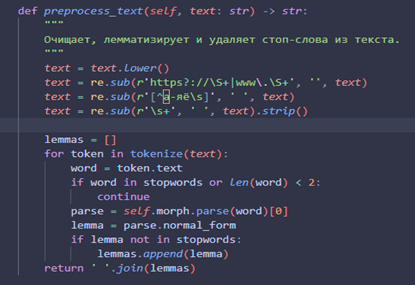
\includegraphics[width=1\textwidth]{styles/diploma/inc/clustulizer1.png} 
    \caption{Предобработка сырого документа}
    \label{fig:example}
\end{figure}

\item  \textbf{Кластеризация:}

 Это центральная часть всего сервиса  ClusterGraphBuilder, в которой «сырые» векторные представления преобразуются в осмысленные кластеры.

На рисунке 16 можно увидеть как:

 \begin{enumerate}[label=\arabic*)] % (1) (2) (3)

 \item  каждый переданный текст в метод предобрабатывается(строка 125);
\item  rаждому тексту сопоставляется его векторное представление с помощью модели  SBERT\_LARGE\_NLU\_RU(строка 129.

 Это переводит тексты из словесного пространства в числовое векторное пространство, благодаря чему можно применять методы машинного обучения;

\item применяется алгоритм HDBSCAN — продвинутый метод плотностной кластеризации, который на основании эмбедингов определяет кластеры и возвращает лейблы кластеров для каждого текста(строки 131-132);
\item пенерируются названия для файлов(строка titles).

\end{enumerate}

\begin{figure}[H]
    \centering
    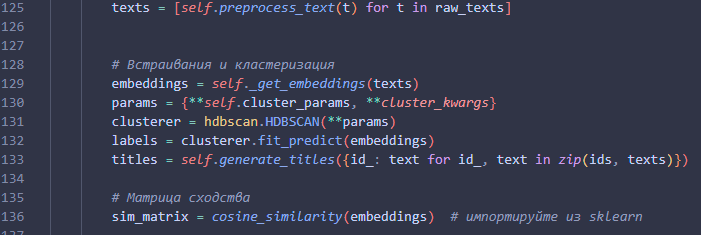
\includegraphics[width=1\textwidth]{styles/diploma/inc/clustulizer2.png} 
    \caption{Кластеризация}
    \label{fig:example}
\end{figure}


\item  \textbf{Представление в виде графа:}

На рисунке 17 представлен код преобразования входных документов в графы.

\begin{figure}[H]
    \centering
    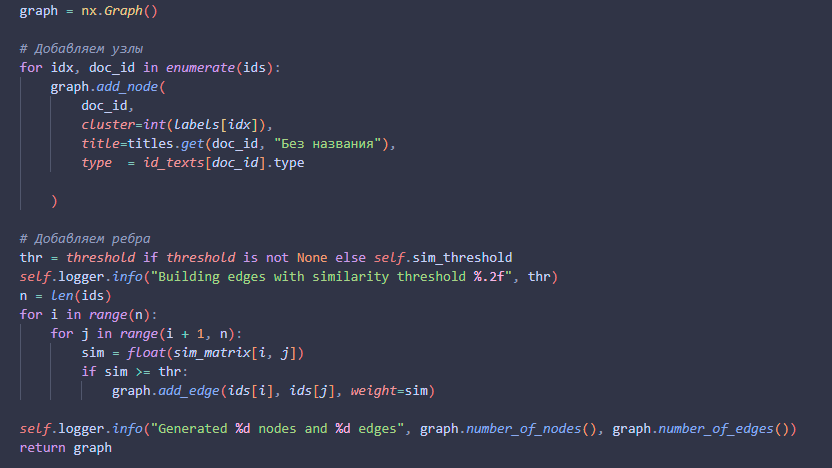
\includegraphics[width=1\textwidth]{styles/diploma/inc/clustulizer3.png} 
    \caption{Кластеризация}
    \label{fig:example}
\end{figure}
\end{itemize}

\clearpage Метод возвращает граф в виде JSON, который имеет вид:

\begin{Verbatim}[fontsize=\small]
{
  "directed": false,
  "multigraph": false,
  "graph": {},
  "nodes": [
    { "id": "Методология ML", "label": "Методология ML" },
    { "id": "Методы ML", "label": "Методы ML" },
    { "id": "Платная рыбалка", "label": "Платная рыбалка" },
    { "id": "Рыбалка Хобби", "label": "Рыбалка Хобби" }
  ],
  "links": [
    { "weight": 0.8477962017, 
    "source": "Методология ML", "target": "Методы ML" },
    { "weight": 0.959409, 
    "source": "Методология ML", "target": "Платная рыбалка" },
    { "weight": 0.768083, 
    "source": "Методология ML", "target": "Рыбалка Хобби" },
    { "weight": 0.784382, 
    "source": "Методы ML", "target": "Платная рыбалка" },
    { "weight": 0.793544,
    "source": "Платная рыбалка", "target": "Рыбалка Хобби" }
  ]
},
\end{Verbatim}
где:
  \begin{itemize}
        \item weight - весь связи, характеризующий, насколько близки 2 вершины;
        \item source, target —  грани, между которыми подсчитан вес.
    \end{itemize}
  

\subsubsection{Handler}
Слой состоит из одного класса  -  RabbitMQServer. Рассмотрит основной метод - обработку входящего сообщения:
 \begin{itemize}
 \item  Микросервис получает сообщение (строчки 61-62);
 \item  Загружает файлы из S3 хранилища (строчка 65);
 \item  Кластеризирует документы  (строчка 69);
 \item  Отправляет результат брокер сообщений   (строчки 73-75).

\end{itemize}

\begin{figure}[H]
    \centering
    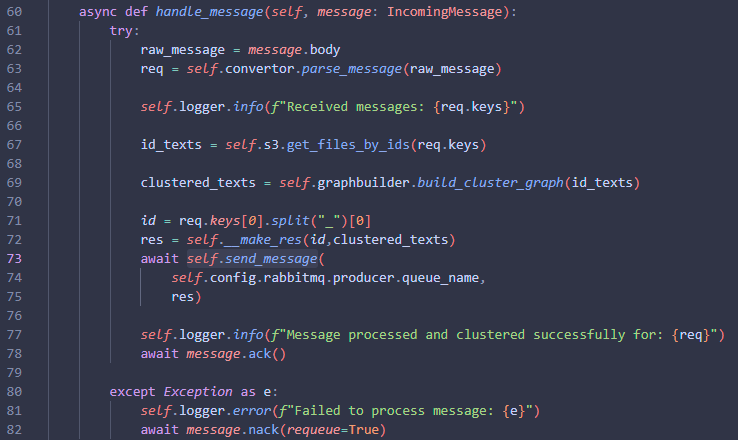
\includegraphics[width=1\textwidth]{styles/diploma/inc/clustulizer_handler1.png} 
    \caption{Метод обработки входящего сообщения на микросервис Clustulizer}
    \label{fig:example}
\end{figure}

\subsubsection{Оценка качества кластеризации и производительности}

Качество кластеризации оценивалось с использованием следующих метрик:

\begin{itemize}
    \item \textbf{Silhouette Score} — показывает, насколько объект внутри кластера схож с другими объектами этого же кластера и отличается от объектов других кластеров. Значение варьируется от $-1$ (плохая кластеризация) до $1$ (идеальная кластеризация), где значения, близкие к $0$, означают наложение кластеров.

    Формула Silhouette Score:
    \begin{equation}
    S = \frac{b - a}{\max(b, a)}  
    \end{equation}
    где:
    \begin{itemize}
        \item $a$ — среднее расстояние до объектов своего кластера;
        \item $b$ — среднее расстояние до объектов ближайшего соседнего кластера.
    \end{itemize}

    \item \textbf{Индекс Дэвиса-Болдина (Davies-Bouldin Index)} — учитывает среднее расстояние между кластерами и их радиусы. Меньшие значения указывают на более чёткие и разделённые кластеры.

    Формула DB Index:
    \begin{equation}
    DB = \frac{1}{n} \sum_{i=1}^{n} \max_{j \ne i} \left( \frac{d_i + d_j}{d_{ij}} \right)
    \end{equation}
    где:
    \begin{itemize}
        \item $d_i$ — среднее расстояние между объектами внутри $i$-го кластера,
        \item $d_{ij}$ — расстояние между центроидами кластеров $i$ и $j$.
    \end{itemize}
\end{itemize}
Тесты проводились на сгенерированных данных с моделированием через KMeans, чтобы колиество лейблов было строго заданным. 
По результатам тестов система показала высокий Silhouette Score и низкий Davies-Bouldin Index: $0.923$ и $0.107$ соответственно, что указывает на эффективность кластеризации большинства документов, тем не менее результаты могут отличаться от реальных данных.

\begin{figure}[H]
    \centering
    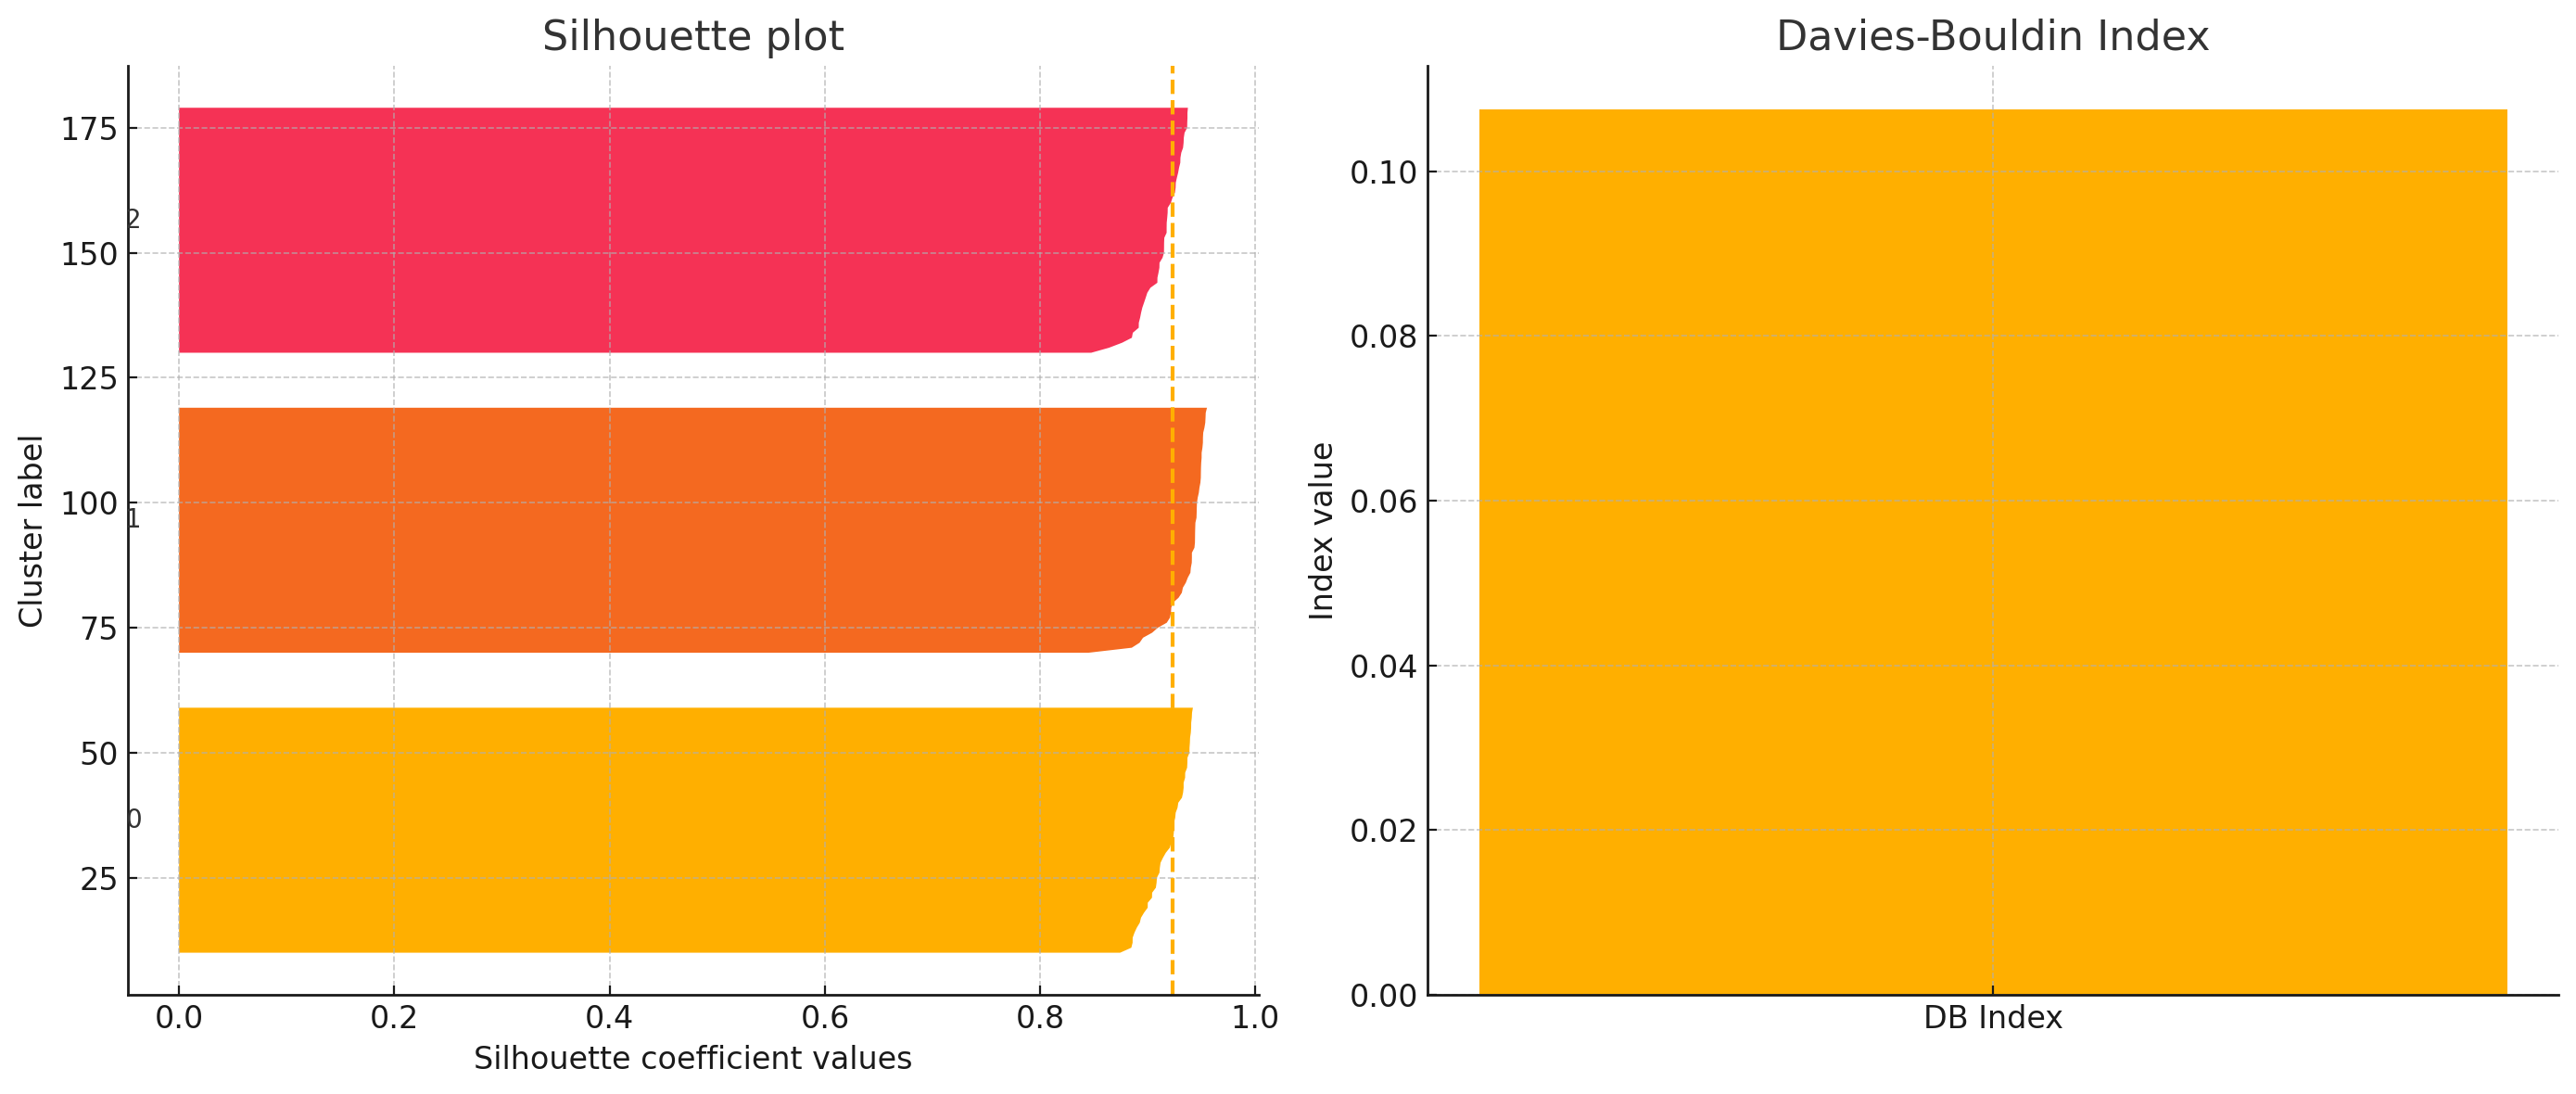
\includegraphics[width=1\textwidth]{styles/diploma/inc/clusturizer_tests1.png} 
    \caption{Результаты тестирования кластеризатора}
    \label{fig:example}
\end{figure}

\vspace{1em}

\textbf{Оценка производительности} проводилась по следующим параметрам: время ответа, пропускная способность, нагрузка на процессор и память. Полученные результаты:
\begin{itemize}
    \item Среднее время ответа — 120 мс;
    \item Загрузка процессора — 60\%;
    \item Пропускная способность — 40 документов в секунду;
    \item Использование памяти — 6 ГБ.
\end{itemize}

\subsection{Пользовательский интерфейс}
Пользовательский интерфейс представляент собой удобную обертку Public API. Для целостного использования сервиса достаточно открытого API, но для пользователя это может доставлять неудобство.
К тому же, интерфейс предсталвяет результат в виде графа, который наглядно показывает, как обработанные документы относятся  к друг другу.

Интерфейс использует ванильный JavaScript, CSS и HTML. Хоть и оформление выглядит минималистично, и если бы использовались другие технологии(например, как ReactJS и HTMX) , оболочка могла смотреться более современно. Однако благодаря этому скорость работы показывает отличные показатели. В будущем приложение обязательно  обзаводется более интересным дизайном с сохранением текущей скорости работы.


\begin{figure}[H]
    \centering
    
\includegraphics[width=1\textwidth]{styles/diploma/inc/front2.png} 
    \caption{Меню загрузки файлов}
    \label{fig:example}
\end{figure}


На рисунке 21 виден результат обработки, введенных пользователем документов. Цветом обозначается кластер. На рисунке 21 2 цвета : синий и желтный. Ребра между вершинами графка показывает, насколько эти вершины близки. Настраивается с помощью матрицы смежности и параметра смежности, который устанавливает уровень, при котором будет отображаться ребро.

 По умолчанию вершины генерируются в виде многогранника, но пользователь имеет возможность двигать вершины.

При нажатии на сгенерированное название для вершины будет скачан файл.

\begin{figure}[H]
    \centering
    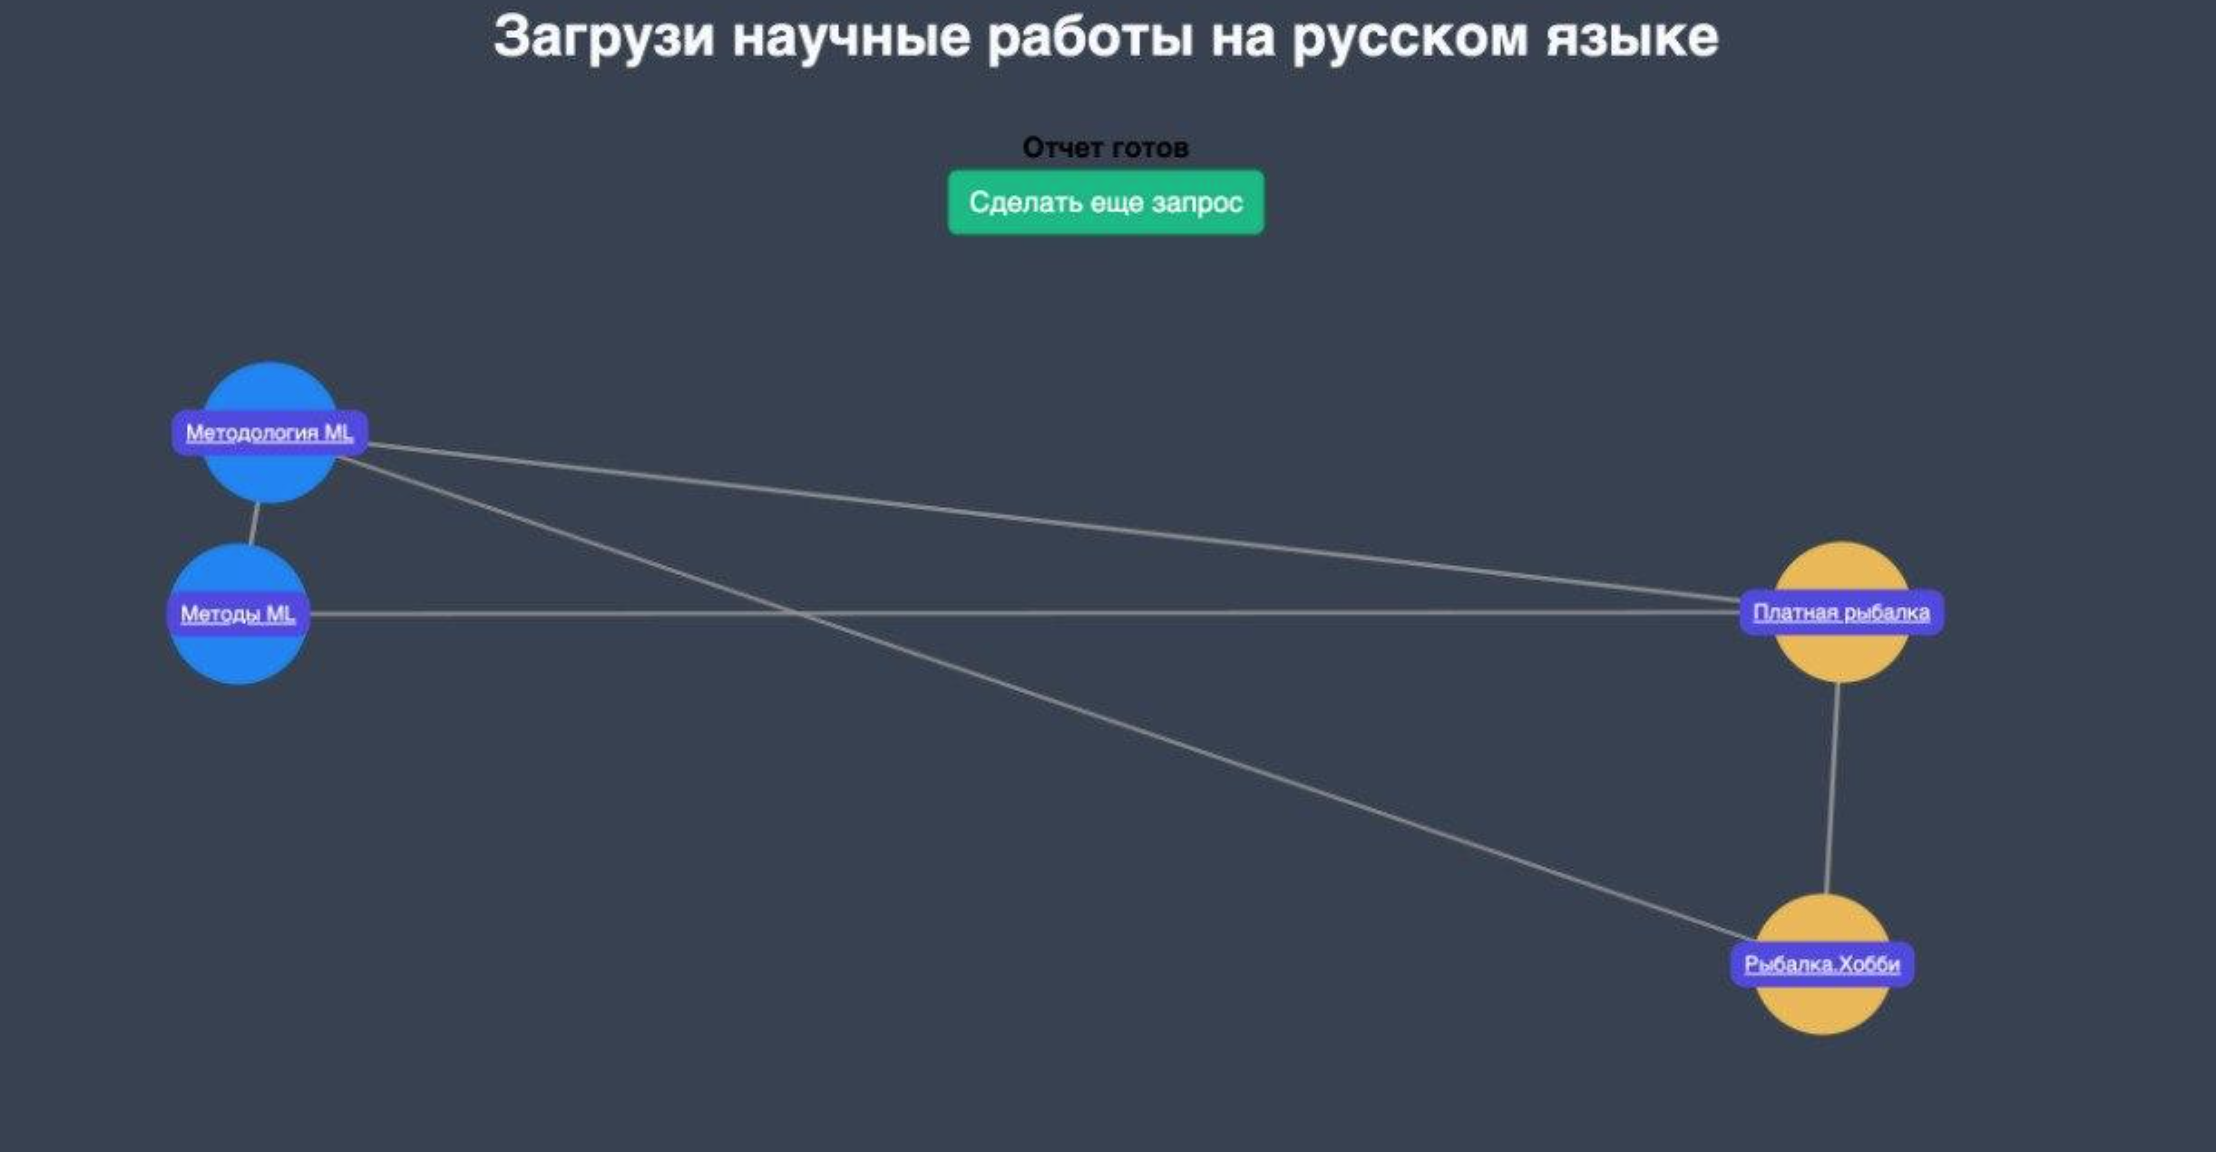
\includegraphics[width=1\textwidth]{styles/diploma/inc/front1.png} 
    \caption{Результат обработки документов}
    \label{fig:example}
\end{figure}